\documentclass[xcolor=table]{beamer}

\usepackage{graphbox}       % For centre alignment of graphics
\usepackage{textcomp}       % Text companion fonts

\setbeamertemplate{navigation symbols}{}
\setbeamertemplate{items}[circle]

\hyphenpenalty 4000 \sloppy


\title{New Tune Fitting Algorithm}
\author{Michael Abbott}
\institute{Accelerator Physics \& Diagnostics Meeting}
\date{Monday 19\textsuperscript{th} February 2018}


\newcommand{\cc}{\cellcolor{green!60!blue!20}}

\begin{document}

\frame{\titlepage}


% ------------------------------------------------------------------------------
%
\begin{frame}{New Tune Fitting Screens}

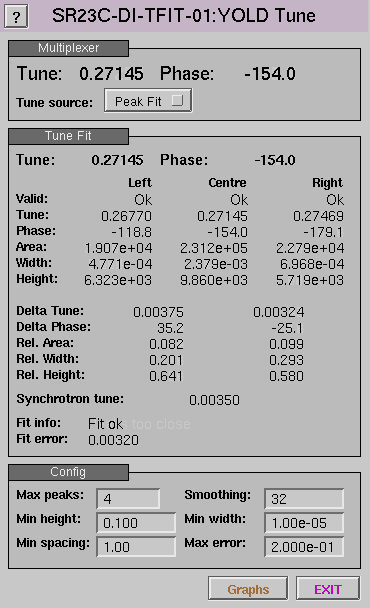
\includegraphics[align=c, width=0.4\linewidth]{tune.png}
\quad
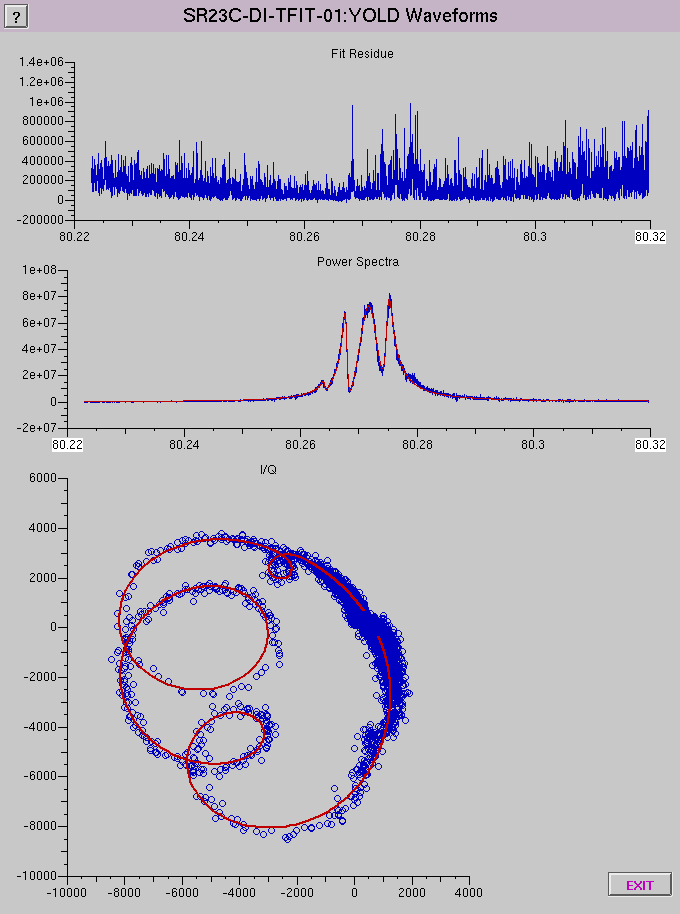
\includegraphics[align=c, width=0.55\linewidth]{graph.png}

\end{frame}


% ------------------------------------------------------------------------------
%
\begin{frame}{Notes on the Measurement}

Table of vertical tune measurement (15\textsuperscript{th} Feb at 08:41)
\medskip

\begin{tabular}{lccc}
 & \cc Left & \cc Centre & \cc Right \\
\cc Tune & 0.26770 & 0.27145 & 0.27469 \\
\cc Width ($\times10^{-4}$) & 4.8 & 23.8 & 7.0 \\
\cc Relative Area & 0.082 & 1.000 & 0.099 \\
\\
\cc Delta Tune & 0.00375 & & 0.00324 \\
\cc Mean Delta & & 0.00350 \\
\cc Synchrotron & & 0.00416 \\
\end{tabular}

\bigskip

Note that the main side bands are much smaller in power (about 10\%) and
narrower (about 25\%) than the centre peak (which we take as the tune).  Also
note that the sideband modulation frequency is about 16\% smaller than the
synchrotron frequency.

\end{frame}


% ------------------------------------------------------------------------------
%
\begin{frame}{Measurement History}
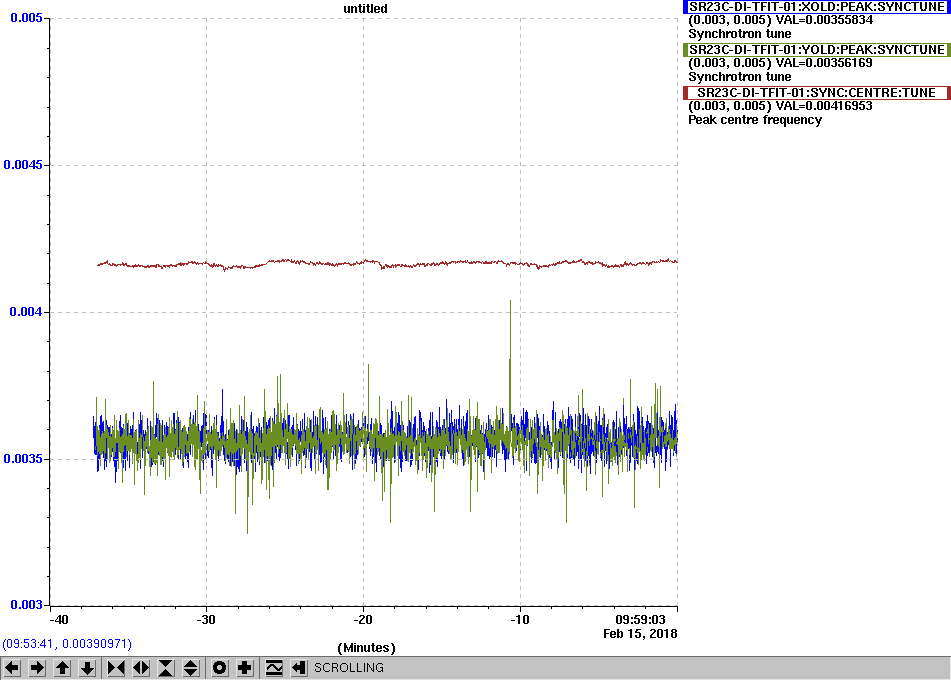
\includegraphics[width=\linewidth]{strip.png}
\end{frame}


% ------------------------------------------------------------------------------
%
\begin{frame}{Fitting Model}
Model raw data
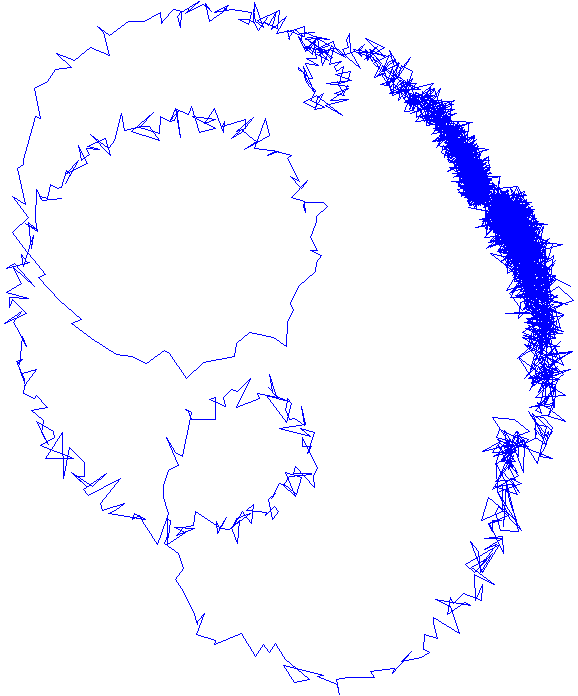
\includegraphics[align=c, width=0.25\linewidth]{raw.png}
as a sum of one pole resonators
\[
    M(\omega) = \sum_{n=1}^N\frac{a_n}{\omega-b_n} + c
              = \frac{P(\omega)}{Q(\omega)}
\]

This is mathematically sound, produces a convincing fit when successful, but is
numerically very difficult to do reliably.

\end{frame}


% ------------------------------------------------------------------------------
%
\begin{frame}{Current (new) Algorithm}
\begin{itemize}
\item Iteratively refine model by adding one peak at a time
    \begin{itemize}
    \item Compute residue by subtracting model so far from raw data
    \item Find largest peak in residual response power by smoothing and looking
        for largest (negative) 2\textsuperscript{nd} derivative
    \item Create initial fit to peak by weighted linear fit around this peak
    \item Use Levenberg-Marquardt refinement to improve the model
    \item Assess quality of model by inspecting each peak
    \item Repeat until enough peaks found or quality of fit is poor
    \end{itemize}
\item Extract three largest peaks from model
\item Take largest peak as tune centre, adjacent peaks (if found) as side-bands
\end{itemize}
\end{frame}


% ------------------------------------------------------------------------------
%
\begin{frame}{Example Fit Failure}

\begin{tabular}{cc}
IQ raw data and models & Pole migration during fit \\
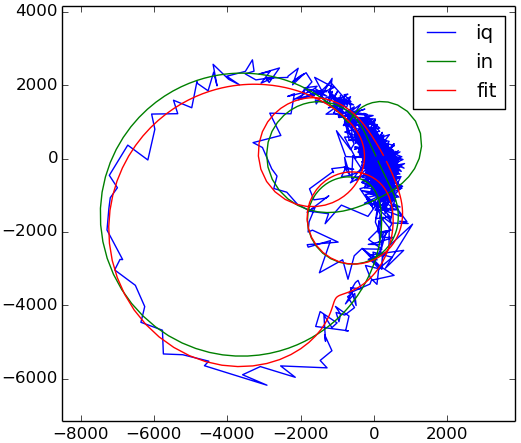
\includegraphics[width=0.4\linewidth]{iq-fit.png} &
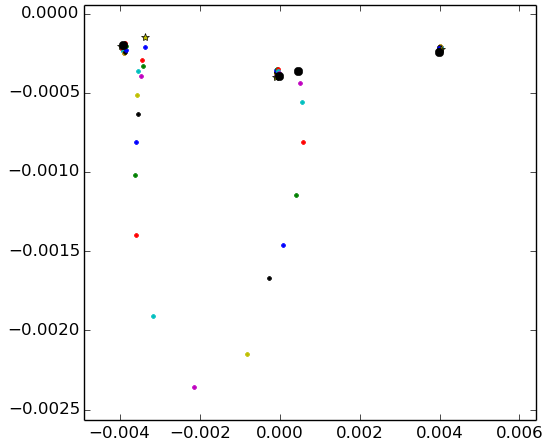
\includegraphics[width=0.4\linewidth]{pole-motion.png} \\
\multicolumn{2}{c}{Power spectrum of fit showing merging peaks (p0, p3)} \\
\multicolumn{2}{c}{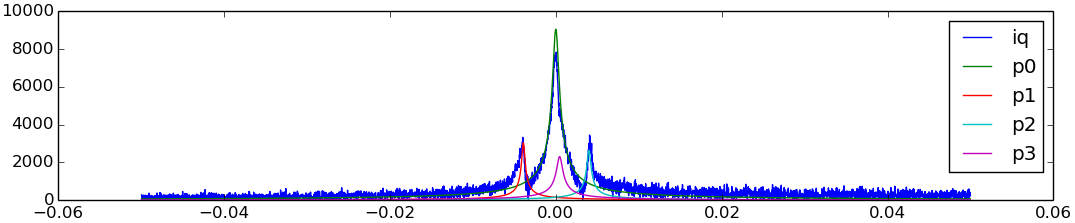
\includegraphics[width=0.9\linewidth]{power-fit.png}} \\
\end{tabular}

\end{frame}

\end{document}
